\documentclass[12pt, a4paper]{article}
\usepackage{array}
\usepackage{longtable}
\usepackage[table]{xcolor}
\usepackage{hyperref}
\usepackage{float}
\usepackage[utf8]{inputenc}
\usepackage{graphicx}
\usepackage{amsmath}
\usepackage{amssymb}
\usepackage{amsfonts}
\usepackage[margin=1 in]{geometry}
\usepackage{color}
\usepackage{caption}
\usepackage{pdflscape}
\usepackage{fancyhdr}

\title{Assignment 2: Foundations\\Statistical Methods for Machine Learning}
\author{Troels Thomsen - qvw203\\Rasmus Haarslev - nkh877\\Allan Martin Nielsen - jcl187}

\setlength\parindent{0pt}		% noindent through whole document
\usepackage[parfill]{parskip}	% extra linebreak on new paragraph

\begin{document}
\pagestyle{empty}
\maketitle
\pagenumbering{gobble}
\newpage

\tableofcontents
\newpage

\pagenumbering{arabic}
\pagestyle{fancy}
\fancyhead[LO,LE]{qvw203 - nkh877 - jcl187}
\fancyhead[RO, RE]{Assignment 2}

\section{II.1.1}
\begin{itemize}
	\item Standard training set error: 0.14
	\item Standard test set error: 0.210526315789
\end{itemize}

We notice that the test accuracy is slightly better than the one found with K-NN in the previous assignment, which was approximately 0.76.

\section{II.1.2}
\begin{itemize}
	\item Normalized training set accuracy: 0.4
	\item Normalized test set accuracy: 0.315789473684
\end{itemize}

We notice a worse result after normalization, which is not quite what we expected. We expected at least the same results, since we are normalizing with a linearly mapping.

Our normalization appears correct however, with the following means and variances for the training set, normalized training set and the data set respectively

\begin{itemize}
	\item Training mean: 
	$\left(\begin{array}{ccc}
		5.7560000000000029 \\
		0.30170000000000008
	\end{array}\right)$
	\item Training variance:
	 $\left(\begin{array}{ccc}
		0.68886399999999981 \\
		0.0017421099999999998
	\end{array}\right)$
	\item Training normalized mean:
	$\left(\begin{array}{ccc}
		-3.4683367289289889e-15 \\
		-1.8174350913113814e-15
	\end{array}\right)$
	\item Training normalized variance:
	$\left(\begin{array}{ccc}
		1.0000000000000004 \\
		0.99999999999999956
	\end{array}\right)$
	\item Test normalized mean: 
		$\left(\begin{array}{ccc}
		0.20837576803933577 \\
		0.43213825772937914
	\end{array}\right)$
	\item Test normalized variance: 
	$\left(\begin{array}{ccc}
		1.0733979533786535 \\
		1.2522227042441971
	\end{array}\right)$
\end{itemize}

Since these appear correct, and since the classifier gives us the correct result on the non-normalized datasets, we are currently unsure as to why we are getting these poor results with the normalized datasets.

\section{II.1.3}
\begin{itemize}
\item \textit{What is its (Bayes optimal) risk?}

We have the two possible hypotheses
\begin{eqnarray}
	h_0(0) &=& 0 \\
	h_1(0) &=& 1
\end{eqnarray}

We can then calculate Bayes optimal risk for these on our set $S$.
\begin{eqnarray}
	\mathcal{R}_S(h) &=& \frac{1}{l}\sum^l_{i=1} \mathbb{I}\{h(x_i) \neq y_i\}
\end{eqnarray}

which gives us the risks

\begin{eqnarray}
	\mathcal{R}_S(h_0) &=& 0.75 \\
	\mathcal{R}_S(h_1) &=& 0.25
\end{eqnarray}

\item \textit{What is the Bayes optimal classifier?}

Bayes optimal classifier is the classifier, that minimizes bayes optimal risk. Hence, \underline{$h_1$} is clearly the Bayes optimal classifier.

\item \textit{What is the risk of the probabilistic classifier?}

The risk of the probabilistic classifier is given by\\
$S_c = \{(0,0),(0,1),(1,0),(1,1)\}$\\
$P(h_{prob}(x)=0) = 0.25\\
P(h_{prob}(x)=1) = 0.75 $
\begin{eqnarray*}
\mathcal{R}(h_{prob}) &=& \sum_{y,z\in S_c} P(Y=y)P(h_{prob}=z)L(y,z)\\ 
\end{eqnarray*}
The first factor is the probability of $y$, one could take $x$ into consideration and make it a joined probability, but since $x$ is always $0$ in this case, we can exclude it.\\
The next factor is the probabilistic classifier, given in the assignment notes and described above.\\
The last factor is the Loss-function.\\\\
And the risk computed with inserted values:
\begin{eqnarray*}
\mathcal{R}(h_{prob}) &=& 0.25 \cdot 0.25 \cdot 0 + 0.25 \cdot 0.75 \cdot 1 +\\
&& 0.75 \cdot 0.25 \cdot 1 + 0.75 \cdot 0.75 \cdot 0 \\
&=& 0.375
\end{eqnarray*}
The risk for the probabilistic classifier is $0.375$
\end{itemize}

\section{II.2.1}
\begin{itemize}
\item \textit{Which of the 3 models provide the best prediction?} 
the RMS for the three selections on the test data are as mentioned:
		\begin{itemize}
		\item \textbf{RMS Selection 1:} 29.9041602819
		\item \textbf{RMS Selection 2:} 28.6056297404
		\item \textbf{RMS Selection 3:} 17.9638970659
	\end{itemize}
\end{itemize}

\begin{figure}[H]
	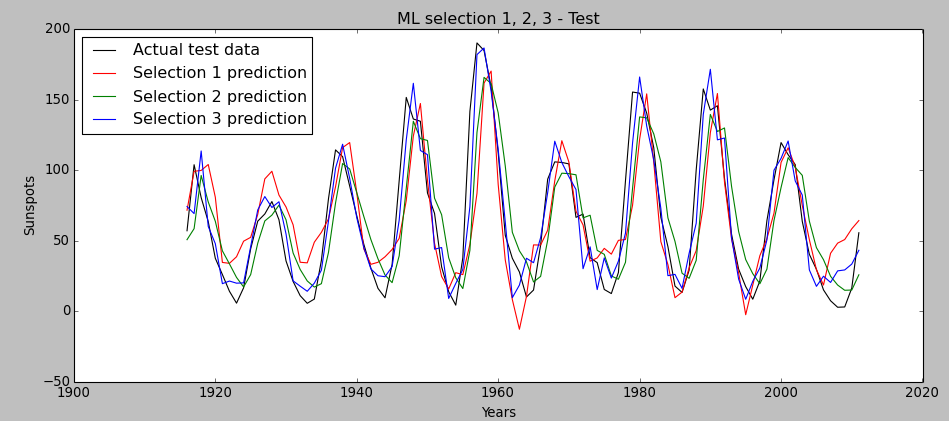
\includegraphics[scale=0.475]{ML_predictions.png}
	\caption{Predictions of all three selections.}
\end{figure}

We see from our figure that selection 3 gives the best fit on the test set, while also having the lowest RMS of 17.9638970659.

\begin{figure}[H]
	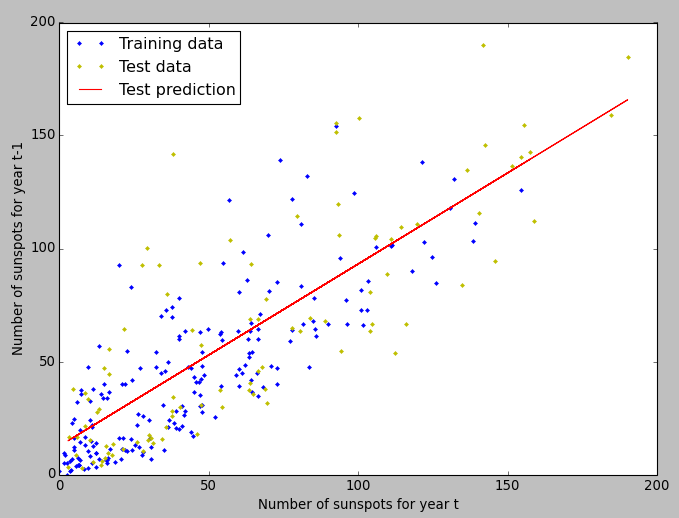
\includegraphics[scale=0.665]{ML_regression.png}
	\caption{Prediction for selection 2, plotted for target against feature.}
\end{figure}

\section{II.2.2}
\begin{itemize}
\item \textit{Which of the three models seem to provide
the best prediction?}
	\begin{itemize}
		\item Like with the ML solution, the 3rd selection using the highest number of years seems to fit the best. This is confirmed by the RMS values.
	\end{itemize}
\item \textit{How do the results compare with the maximum likelihood
results?}
	These are our RMS results for $\alpha = 0.5$
	\begin{itemize}
		\item \textbf{RMS for map selection1:} 29.9112229729
		\item \textbf{RMS for map selection2:} 28.6058321345
		\item \textbf{RMS for map selection3:} 17.9664239687
	\end{itemize}
\item \textit{For what value of the prior precision parameter $\alpha$ does the RMS error go below the RMS for the maximum likelihood solution from Question II.2.1?}
	\begin{itemize}
		\item We could not find an $\alpha$ for which the RMS for MAP was lower than that found in our ML solution. As expected we came closer and closer to $RMS_{ML}$ when $\alpha$ approached 0, but as we increased $\alpha$, so did our $RMS_{MAP}$ and as such we could not improve on the results found with the ML solution.
	\end{itemize}
\end{itemize}

\section{II.2.3}
\begin{itemize}
\item \textit{Find an expression for the solution $\textbf{w}^*$ that minimizes this error function.}

To minimize the error function, we differentiate it, set it equal to 0, and then isolate w.

\begin{eqnarray}
	\frac{\delta E_D}{\delta w} &=& \frac{1}{2}\sum^N_{n=1}(2r_n(t_n - w \phi (x_n))(-\phi^T (x_n))\\
	0 &=& \frac{1}{2}\sum^N_{n=1}(2r_n(t_n - w \phi (x_n))(-\phi^T (x_n))\\
	0 &=& \frac{1}{2}\sum^N_{n=1}(2r_nt_n - 2r_nw \phi (x_n))(-\phi^T (x_n))\\
	0 &=& \frac{1}{2}\sum^N_{n=1}2r_nt_n\phi^T (x_n) + 2r_nw \phi (x_n) \phi^T (x_n)\\	
	0 &=& \sum^N_{n=1}r_nt_n\phi^T (x_n) + r_nw \phi (x_n) \phi^T (x_n)\\
	0 &=& \sum^N_{n=1}(r_nt_n\phi^T (x_n)) + \sum^N_{n=1}(r_nw \phi (x_n) \phi^T (x_n))\\
	0 &=& \sum^N_{n=1}(r_nt_n\phi^T (x_n)) + w\sum^N_{n=1}(r_n \phi (x_n) \phi^T (x_n))\\
	-\sum^N_{n=1}(r_nt_n\phi^T (x_n)) &=& w\sum^N_{n=1}(r_n \phi (x_n) \phi^T (x_n))\\
	\frac{-\sum^N_{n=1}(r_nt_n\phi^T (x_n))}{\sum^N_{n=1}(r_n \phi (x_n) \phi^T (x_n))} &=& w
\end{eqnarray}


\item \textit{Give two alternative interpretations of the weighted sum-of-squares
error function in terms of}
\begin{itemize}

	\item We wish to choose $r_n$ in such a way that it compliments our data. For noisy data we can pick $r_n$ such that we give larger errors for larger deviations. We could for instance weigh with the error squared, as in the root-mean-squares error function. This would punish larger deviations more severely than smaller ones, thereby hopefully correcting some of the noisiness. 
	\item For data with replicated data points we can pick $r_n$ such that we divide the error with the number of replications. In this way replicates will on average have the same impact on the regression, as if they were one point.
 
\end{itemize}
\end{itemize}

\end{document}

